\chapter{The Camera Module}

Cameras are the interface between images and the real world, and as
such, their importance in computer vision cannot be understatetd.  In
fact, some would say that computer vision algorithms are distinguished
by the fact that they endeavor to associate the processed pixel data
with objects in the real world for the purposed of measurement,
tracking, or display.  This is achieved by modeling the geometric and
physical properties of the device that was used to capture the
original image.  This is the purpose of the camera module.

The camera module includes built-in models for generic pinhole and
line-scan imagers and a set of generic functions for linearizing
(removing lens distortion) and epipolar rectifying (e.g. for stereo)
when these operations are relevant.  These classes and functions can
be imported into your code by including {\tt <vw/Camera.h>}.

Because you will likely encounter new camera geometries not supported
by the built-in classes, the camera module is designed to be
extensible: the user can provide their own camera model by inheriting
from and adopting the interface of the {\tt CameraModel} abstract base
class in {\tt <vw/Camera/CameraModel.h>}.

Finally, the camera module provides a basic set of tools for working
with images from real-world camera systems: bayer pattern filtering
and EXIF parsing.  We will cover all of these features in more detail,
however we begin this chapter by establishing some terminology whilst
exploring the most common camera geometry in use today: the pinhole
camera model.

\section{The Pinhole Camera Model}
The pinhole camera model describes the geometry found in nearly all
commercial digital camera systems today.  It is characterized by a
lens assembly that focuses light onto a two dimensional array of
pixels (usually a sensor with light sensitive circuits such as a CCD
or CMOS device).  We will use the pinhole model to establish some
terminology that will be used throughout the rest of this chapter.  Be
warned that the model we are about to develop is simplistic; many of
the non-ideal characteristics of a real-world optical system
(e.g. lens distortion) are not modeled in this simple example.  Refer
to the CAHVOR model in Section \ref{sec:built-in-cameras} if you
require a pinhole camera model that more accurately models lens
distortion.

\subsection{Perspective Projection}

Figure \ref{fig:pinhole-camera-diagram} shows the geometry of a basic
pinhole camera.  The light gray area represents the 2D array of
pixels, and it is referred to as the {\em image plane}.  The origin of
the 3D coordinate system is the point $C$, which is the center of
projection or {\em camera center} of the imager.  When a 3D point $O$
is imaged by the camera, it appears at the pixel located where segment
$\overline{OC}$ intersects the image plane at point $(u,v)$.  A line
segment $\overline{OC}$ that is perpindicular to the image plane
intersects this plane at the {\em principal point}, $(p_u, p_v)$.

\begin{figure}[tbp]
\begin{center}
  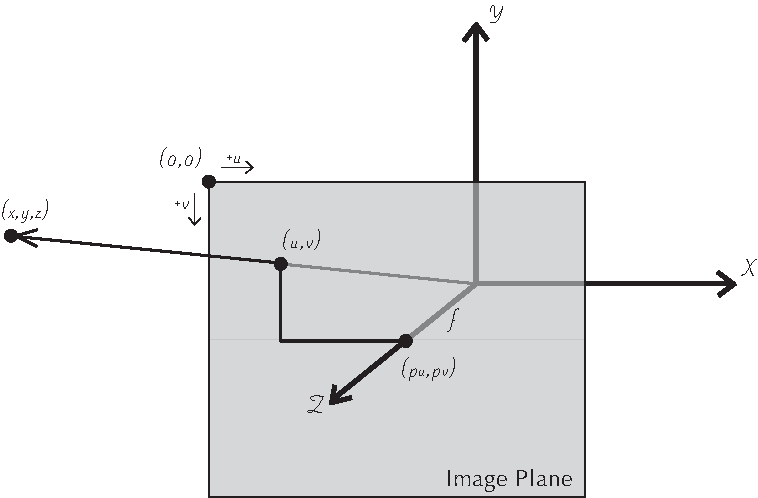
\includegraphics[width=6in]{images/camera_module_pinhole.pdf}
 \end{center}
  \caption{The basic pinhole camera model.}
  \label{fig:pinhole-camera-diagram}
\end{figure}

All of the points imaged by the camera appear on a line that passes
through $C$.  If the coordinates of ${\bf O}$ are $(x,y,z)$, then the
position of the point on the imager can be determined by projecting it
onto the plane $ z = +f$:
\begin{eqnarray}
\label{eqn:forward-projection-1}
u &=& \frac{f}{\sigma} \left(\frac{x}{z}\right) - p_u \\
\label{eqn:forward-projection-2}
v &=& \frac{f}{\sigma} \left(\frac{-y}{z}\right) - p_v
\end{eqnarray}

Here, $f$ is the focal length of the imager in meters, $\sigma$ is the
size of a pixel in {\em m/pixel}, and $(p_u, p_v)$ are the offset in
pixels of the principal point (this offset moves the origin of the
image from the principal point to the upper left hand corner, which is
the ``origin'' usually adopted when indexing images).  

Equations \ref{eqn:forward-projection-1} and
\ref{eqn:forward-projection-2} consitute the {\em forward projection}
portion of the camera model; this is analogous to the process of
``capturing'' an image with a real camera.  Our model should tell us
exactly what what pixel location to look at if you wanted to see the
point $O$ in the image.

Notice how some information is lost during forward projection.  Any
point along $\overline{OC}$ will be imaged to the same point $(u,v)$
on the image plane, so if we were to start with a point $P=(u,v)$ on
the image plane, and we wanted to find the original 3D point $O$, the
best we could do would be to say that it appears somewhere along the
ray $\overrightarrow{CP}$. The
origin and direction of the ray can be computed as follows:

\begin{eqnarray}
\label{eqn:reverse-projection-1}
\overrightarrow{CP}_{origin} & = & C \\
\label{eqn:forward-projection-2}
\overrightarrow{CP}_{direction} & = & \frac{(u + p_u, -(v + p_v), f)} {||(u + p_u, -(v + p_v), f)||_2}
\end{eqnarray}

This operation, which we call {\em back projection}, can still
provide useful inforamation that can be used in a full 3D
reconstruction despite the ambiguity in the actual postion of $O$.
Imagine that you have two cameras that have imaged the same point $O$
from two different viewpoints at pixel locations $P_1$ and $P_2$ in
their respective image planes.  Using simple geometry, you can
reconstruct the position of $O$ by computing the intersection of the
two rays emanating from each camera center through $P_1$ and $P_2$.
This is the technique commonly referred to as stereo reconstruction,
and it is one of the many ways that you can make use of the
information provided by back projection.

\section{The Camera Model Base Class}

As we have seen, a camera model provides a means for forward
projection (``imaging'' 3D points onto a 2D array of pixels) and back
projection (finding the ray along which a 3D points must lie given a
2D pixel where it was imaged).  All camera models in the Vision
Workbench derived from the CameraModel abstract base class, which
enforces this basic interface.

Forward projection of a 3D point is handled by the
\verb#point_to_pixel()# method.
\begin{verbatim}
  CameraModel* camera_model = new MyDerivedCameraModelClass;
  Vector3 world_coordinates;
  Vector2 pixel_coordinates = camera_model.point_to_pixel(world_coordinates);
\end{verbatim}
Remember that in C++, you will need to maintain a pointer to the
derived camera model class in order to ensure that the virtual
inheritance mechanism calls the method from the derived class rather
than the base class.

The back projection operation is split into two seperate API calls.
The \verb#camera_center()# method returns the origin of the ray, and
the \verb#pixel_to_vector()# method returns its direction.  Remember
that any of the points that lie along this ray would have been imaged
at $(u,v)$, so this pixel-to-ray operation leaves some ambiguity about
the true location of the point $O$.
\begin{verbatim}
  CameraModel* camera_model;  
  Vector3 ray_origin = camera_model.camera_center(pixel_coordinates);
  Vector3 ray_direction = camera_model.pixel_to_vector(pixel_coordinates);
\end{verbatim}
\begin{center}\fbox{\parbox{7in}{
{\bf Camera Coordinate Systems}\\ \\ Vision Workbench camera model
classes take and return coordinates that are {\em not} homogeneous.
That is, coordinates do not need to augmented with an additional
homogeneous scaling element before being passed to camera module
routines (e.g. a 2D vector $(325, 206)$ in cartesian coordinates is
often represented as $(325, 206, 1)$ in homogeneous coordinates).
Homogeneous coordinates have certain advantages in projective geometry
(e.g. they allow a tranlation of the coordinates to be encoded as a
matrix multiplication), however we have chosen not to adopt this
convention.}}
\end{center}

\section{Built-in Camera Models}
\label{sec:built-in-cameras}
The Vision Workbench comes with several ``built-in'' camera models.
These classes satisfy the needs of most common applications, and they
can also serve as a design reference for your own camera model
classes.  Each class models a specific geometry and, to varying
extents, the non-ideal characteristics of the camera system such as
lens distortion.

The list of built-in models are summarized in Table
\ref{tab:camera-models}.  The following sections describes the two
basic classes of built-in camera model: those that model pinhole
cameras (where the imager is a 2D array of pixels), and those that
model linescan cameras (where the imager is a 1D line of pixels).

\begin{table}[tdp]
\begin{center}
\begin{tabular}{|l|l|l|l|}
\hline
{\em Camera Model} & {\em Header File} & {\em Imager Type} & {\em Details}\\
\hline CAHV         & {\tt CAHVModel.h} & Pinhole     & Basic pinhole camera model \\
CAHVOR       & {\tt CAHVORModel.h} & Pinhole     & Models lens distortion\\
Linescane     & {\tt LinescanCameraModel.h} & Linescan & Generic Linescan Model \\
Linear Pushbroom    & {\tt LinearPushbroomModel.h} & Linescan & Assumes linear flight path \\
Orbiting Pushbroom & {\tt OrbitingPushbroomModel.h} & Linescan & Models curvature of orbit \\
\hline
\end{tabular}
\end{center}
\label{tab:camera-models}
\caption{Built-in camera models can be found in {\tt vw/Camera/} }
\end{table}

\subsection{Pinhole Cameras}

The {\em CAHV camera model} has been widely used in NASA planetary
mission for rover navigation and scientific camera systems
\cite{yakimovsky78}.  It is a basic pinhole camera model that does not
model lens distortion or other optical aberrations.  The CAHV model is
so named because the camera intrinsic and extrincsic parameters are
jointly parameterized by four 3-dimensional vectors: C,A,H, and V.
This compact represenation leads to a very efficient forward
projection operation, which is the strength of the CAHV model.
Forward projection of a real world point $O$ can be computed using

\begin{eqnarray}
u & = & \frac{(O-C) \cdot H}{(O-C) \cdot A}\\
v & = & \frac{(O-C) \cdot V}{(O-C) \cdot A}
\end{eqnarray}

The user has two choices when initializing a CAHV camera model.
First, they can construct the object by directly supplying four
3-vectors to the constructor.

\begin{verbatim}
  Vector3 C,A,H,V;
  CameraModel* cam = new CAHVModel(C,A,H,V);
\end{verbatim}

Alternatively, users seeking to use the CAHV class as a general purpose pinhole
camera model may find it easier to use the more verbose constructor
wherein the camera extrinsics and intrinsics are explicitly supplied.

\begin{verbatim}
  double focal_length;
  Vector2 pixel_size;
  double principal_point_h, principal_point_v;
  Vector3 camera_center, pointing_vector;
  Vector3 horizontal_vector, vertical_vector; // Defines image plane orientation

  CameraModel* cam = new CAHVModel(focal_length, pixel_size, principal_point_h, 
                                   principal_point_v, camera_center, 
                                   pointing_vector, horizontal_vector,
                                   vertical_vector);  
\end{verbatim}


The {\em CAHVOR model} is an expanded camera model with two additional
3-vectors (O and R) that describe lens distortion introduced by the
camera lens.

Refer the Doxygen-generated API documentation for more information
about constructing CAHV and CAHVOR camera models.

\subsection{Linescan Cameras}

Linescan imagers capture images using a sensor containing a
1-dimensional array of pixels.  The image is formed by capturing
successive scan-lines as the camera platform is rotated or moved.  For
example, a flat-bed scanner or photocopier is a familiar example of
such a system.  The sensor is swept in the so-called {\em along-track}
direction along the document, composing the final image by
concatenating several thousand adjacent 1-dimensional images taken at
evenly spaced positions.

Linescan sensors are fairly uncommon in commercial camera systems, but
they appear frequently on satellites that capture photographs of
terrain from orbit.  The orbital motion of the satellite is used in
much the same way as the motion of the sensor in the photocopier; the
{\em across-track} dimension of the image corresponds to the
projection of 3D points through the lens onto the sensor, and the
along-track dimension of the image corresponds to successive scanlines
taken at different times as the satellite moves.

\begin{figure}[tbp]
\begin{center}
  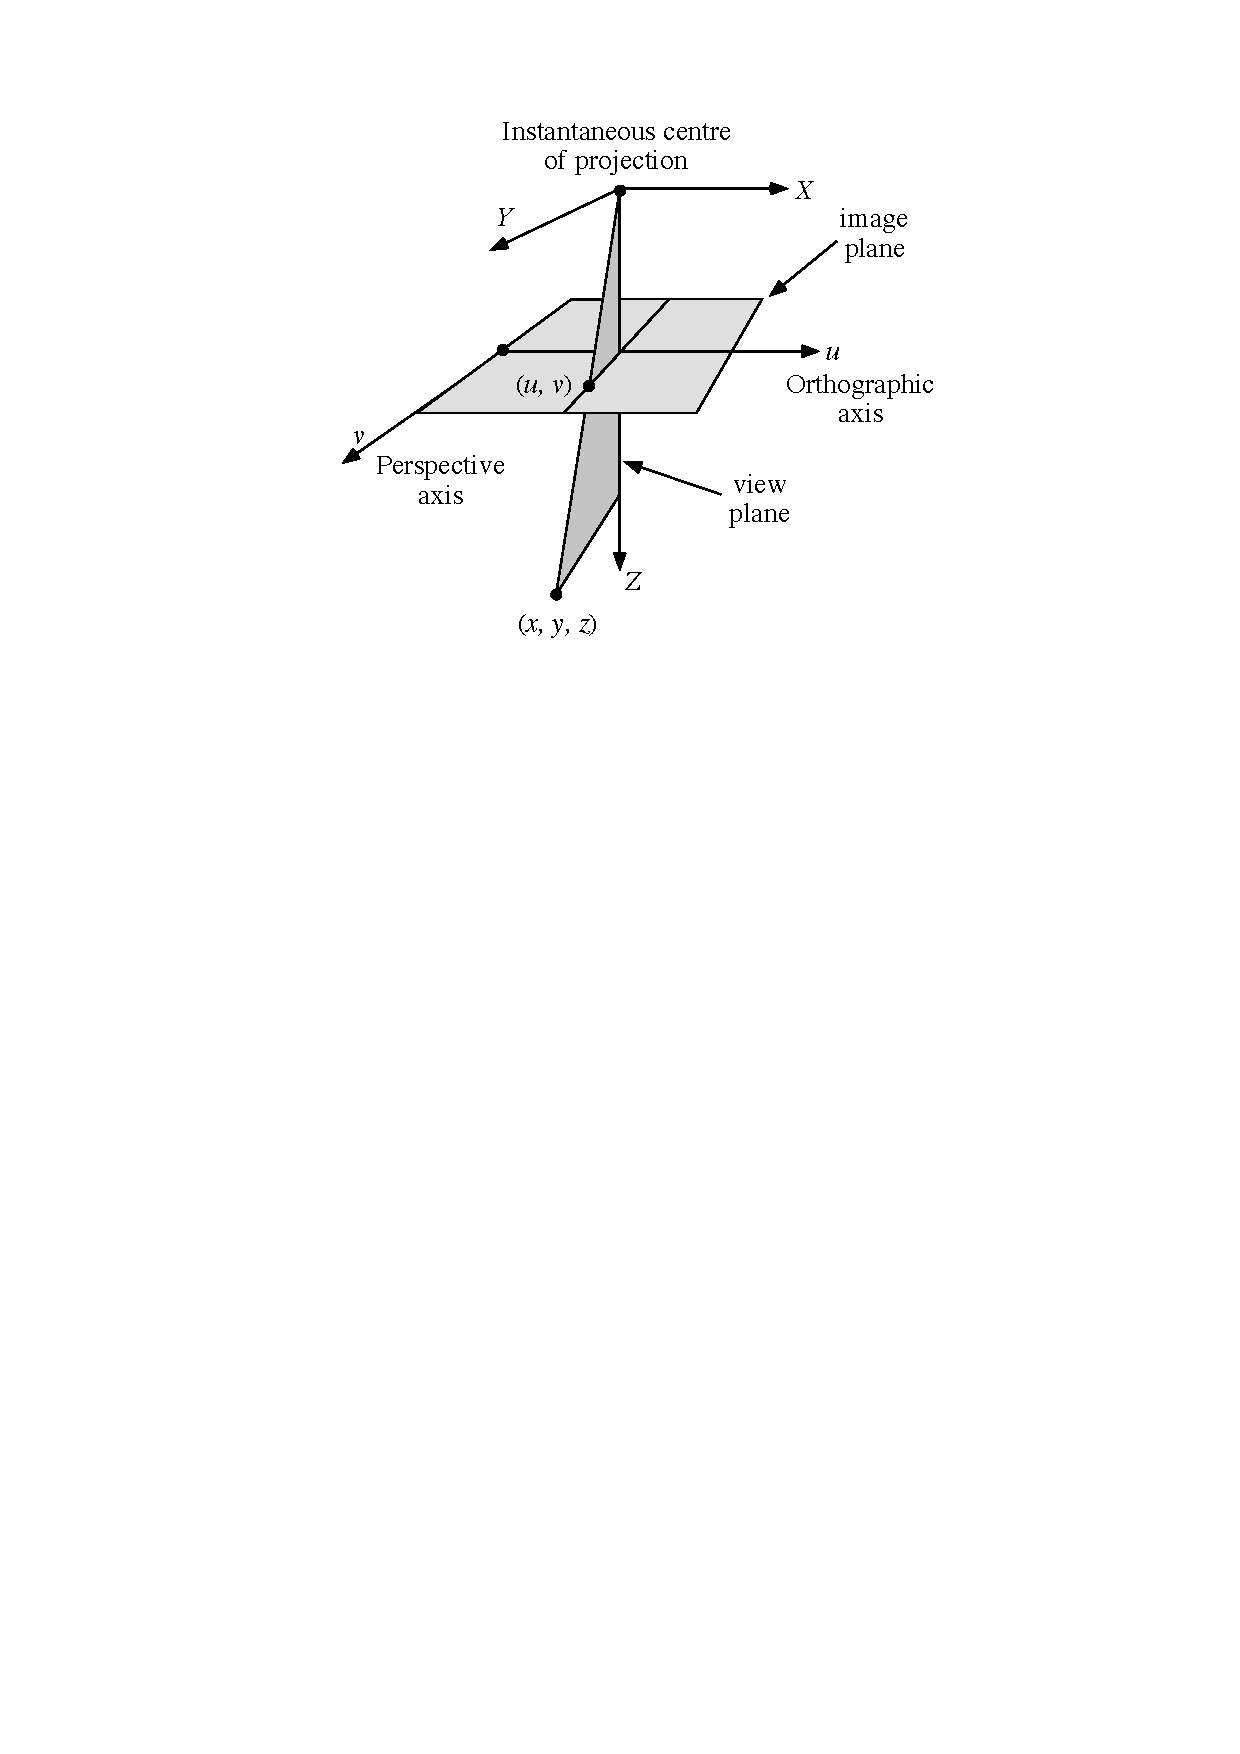
\includegraphics[width=5in]{images/pushbroom_geometry.pdf}
 \end{center}
  \caption{Geometry of the Linescan Camera Model.}
  \label{fig:linescan-geometry}
\end{figure}

The geometry of the linescan imager is subtly different from the
geometry of the pinhole camera.  See Figure
\ref{fig:linescan-geometry}.  Although there is still a center of
projection created by the camera's optics (and points are still imaged
using a perspective projection in the across-track direction), this
point moves as the camera moves, and as a result, the along-track
position of a pixel in a linescan image is purely a function of the
position and orientation of the camera; both a function of time.  The
orientation of the image (in the sense that $u$ indexes the columns of
an image and $v$ indexes its rows) must be chosen consistent with
Figure \ref{fig:linescan-geometry} when working with
\verb#LinescanModel# and its relatives.

In the special case where the motion of the linescan sensor is linear
and its orientation is fixed, the projection of the points onto the
image in the along-track is orthographic.  These assumptions are the
basis for the {\em Linear Pushbroom Model}, which can be found in
\verb#<vw/Camera/LinearPushbroomModel.h>#.  If you are interested in
understanding this model in detail, we recommend you read the
excellent paper by Gupta and Hartly \cite{gupta97}.

If you must relax the assumption about a linear filght path somewhat
to allow sensor pose to vary and the camera motion to lie along a
curve (as is common with orbiting camera systems), the {\em Orbiting
  Pushbroom Model} is an appropriate choice.  In the Orbiting
Pushbroom model, the user supplies a series of evenly spaced samples
of position and orientation and specifies the time interval (in
seconds) between samples.  A sparse set of samples is sufficient for
this model: interpolation occurs for points in between the supplied
positions and orientations.

\section{Tools for Working With Camera Images}

This section describes several tools that simplify the process of
working with image captured by real cameras.

\subsection{Inverse Bayer Pattern Filtering}

Most imaging sensors are inherently grayscale capture devices.  In
order to capture color, some imagers have a hardware color filter
placed in front of the pixels on the CCD.  This is called a {\em Bayer
  filter}.  The Vision Workbench provides the
\verb#inverse_bayer_filter()# method in
\verb#<vw/Camera/BayerFilter.h># converting the raw, grayscale pixel
values from the sensor and producing a color image by interpreting the
Bayer filter effect.

\subsection{Exif Exposure Data}

Digital cameras store data about the settings used to take a picture
in the image file according to the EXIF standard \cite{exif}. EXIF
data is stored using the Image File Directory system described in the
TIFF 6.0 standard.  EXIF tags such as {\tt FNumber} and
{\tt ExposureTime} can be useful for radiometrically calibrating your
camera images.  Unfortunately the standard is redundant and often
poorly supported by camera manufacturers (for example, many hide the
ISO setting in the maker note instead of storing it in the
ISOSpeedRatings tag), so we cannot gurantee support for every camera.

The Camera module includes the {\tt ExifView} class (defined in
\verb#<vw/Camera/Exif.h>#) for extracting this data from images.  To
create this class, you supply the filename of an image on disk.
Currently, JPEG and TIFF images are supported.  ExifData and ExifView
were based on {\tt jhead}, an EXIF JPEG header and thumbnail manipular
program in the public domain \cite{jhead}.

\begin{verbatim}
  // Reliably get F number. 
  ExifView view;
  if (view.load_exif(``img.jpg'')) {
    double f = view.get_f_number();
    // ...
  }
\end{verbatim}

\begin{thebibliography}{1}

\bibitem{exif} ``Exchangeable image file format for digital still cameras: Exif Version 2.2'',
(Japan Electronics and Information Technology Industries Assocation, 2002),
http://www.exif.org/specifications.html.

\bibitem{gupta97} Gupta, Rajiv and Hartley, Richard. ``Linear Pushbroom Cameras''.  IEEE
 Transactions on Pattern Analysis and Machine Intelligence. Vol.19 No. 9. September 1997

\bibitem{jhead} Wandel, Matthias, ``Exif Jpeg header and thumbnail manipulator program,'' 2006,
http://www.sentex.net/~mwandel/jhead/.

\bibitem{yakimovsky78}  Yakimovsky, Y. and Cunningham R., ``A System for Extracting
  Three-Dimensional Measurements from a Stereo Pair of TV Cameras ''
  Computer Graphics and Image Processing 7, pp. 195-210. (1978)

\end{thebibliography}
